\documentclass[conference]{IEEEtran}

\usepackage{cite}
\usepackage{amsmath,amssymb,amsfonts}
\usepackage{graphicx}
\usepackage{textcomp}
\usepackage{xcolor}
\usepackage{booktabs}
\usepackage{multirow}
\usepackage{url}

\graphicspath{{../figures/}{../checkpoints/baseline_v2/}}

\begin{document}

\title{Robust Contactless Palmprint Verification with Deep Metric Learning: Checkpoint Report}

\author{
\IEEEauthorblockN{Huy Ong}
\IEEEauthorblockA{CS 228 -- Biometric Security\\Spring 2026}
}

\maketitle

\begin{abstract}
Contactless palmprint verification offers a hygienic and user-friendly biometric modality, but real-world capture variations such as noise, motion blur, and lighting changes can severely degrade system performance. In this work, we develop a verification system using ResNet18 with ArcFace angular margin loss, trained and evaluated on the PolyU--IITD contactless palmprint dataset (611 subjects, 12,220 images) with subject-disjoint splits. Our baseline achieves an Equal Error Rate (EER) of 1.67\% on clean test data. A systematic robustness benchmark across 9 corruption types at 5 severity levels reveals that noise (+1,170\%), motion blur (+1,041\%), and brightness variations (+796\%) cause the most severe degradation, while contrast and scale changes remain manageable.
\end{abstract}

% ============================================================
\section{Refined Problem Statement and Motivation}

Contactless palmprint verification is an emerging biometric modality that captures palm images without physical contact, improving hygiene and user acceptance compared to fingerprint sensors. Palmprints contain rich discriminative features---principal lines, wrinkles, and texture patterns---that remain stable over time, making them well-suited for identity verification.

However, contactless capture introduces challenges absent in contact-based systems. Variations in hand pose, sensor distance, ambient lighting, motion blur, and compression artifacts all affect image quality. A practical verification system must not only achieve high accuracy on clean images but also degrade gracefully under these real-world conditions. When performance degrades, both security (increased false accepts) and usability (increased false rejects) are compromised.

This project addresses the question: \textit{How robust is a deep learning-based palmprint verification system to common real-world capture variations, and which factors pose the greatest risk to deployment?}

\subsection{Scope Changes from Proposal}

{\color{blue}
The following changes have been made relative to the original proposal:
\begin{itemize}
    \item \textbf{Dropped:} MobileNetV3 backbone comparison---we focused on ResNet18 to invest effort in a thorough robustness benchmark instead.
    \item \textbf{Completed:} Full robustness benchmark across 9 corruption types $\times$ 5 severity levels (45 conditions), exceeding the originally planned 4--6 types.
    \item \textbf{Deferred:} Mitigation implementation (robust augmentation training or quality gating) is deferred to the final phase of the project.
\end{itemize}
}

% ============================================================
\section{Data Engineering and Provisioning}

\subsection{Dataset}

We use the \textbf{PolyU--IITD Contactless Palmprint Database v3.0}~\cite{polyu}, comprising 611 subjects with 20 images each (10 left hand + 10 right hand), totaling 12,220 images. All images are 128$\times$128 grayscale ROI-cropped palmprint regions.

\subsection{Preprocessing}

Each grayscale image is converted to 3-channel RGB for compatibility with ImageNet-pretrained backbones. Images are normalized using ImageNet channel statistics ($\mu = [0.485, 0.456, 0.406]$, $\sigma = [0.229, 0.224, 0.225]$). During training, we apply data augmentation including random cropping, horizontal flipping, rotation ($\pm$15\textdegree), color jitter, Gaussian blur, and random erasing to improve generalization.

\subsection{Subject-Disjoint Splits}

To prevent identity leakage, we use subject-disjoint splits where no subject appears in more than one partition. Each (subject, hand) combination is treated as a unique class, doubling the effective number of identities:

\begin{table}[h]
\centering
\caption{Dataset splits with subject-disjoint protocol.}
\label{tab:splits}
\begin{tabular}{lccc}
\toprule
\textbf{Split} & \textbf{Subjects} & \textbf{Images} & \textbf{Classes} \\
\midrule
Train      & 427 (70\%) & 8,540  & 854 \\
Validation & 61 (10\%)  & 1,220  & 122 \\
Test       & 123 (20\%) & 2,460  & 246 \\
\bottomrule
\end{tabular}
\end{table}

A quality audit identified 4 empty placeholder subjects (H\_ID608--611) in the original dataset; these were excluded from all splits.

\begin{figure}[t]
\centering
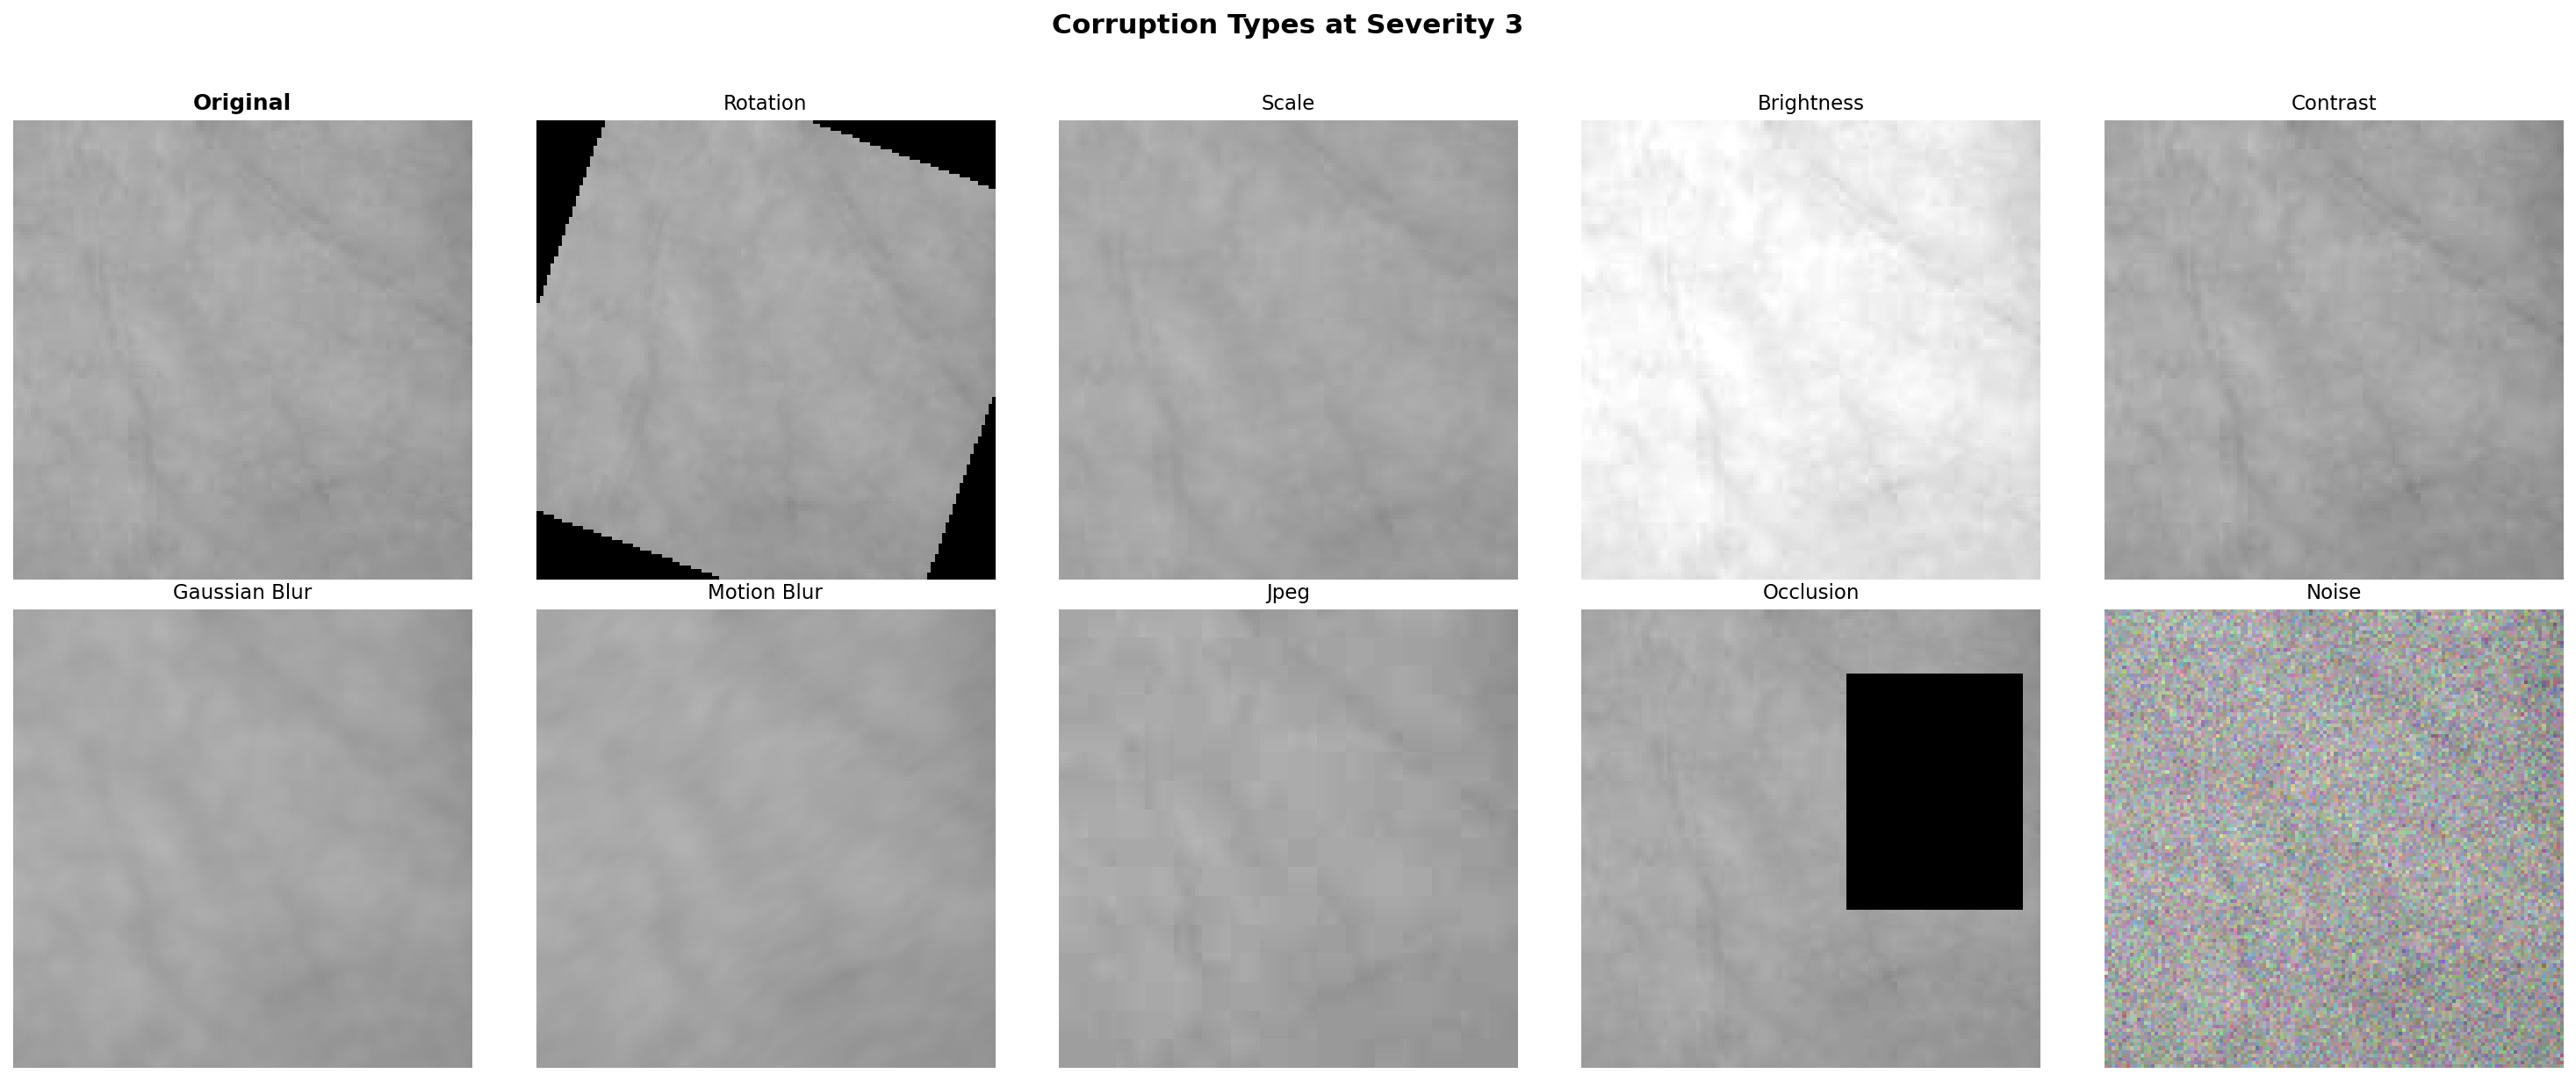
\includegraphics[width=\columnwidth]{corruption_samples.png}
\caption{Original palmprint image and 9 corruption types at severity level 3. Top row: Original, Rotation, Scale, Brightness, Contrast. Bottom row: Gaussian Blur, Motion Blur, JPEG, Occlusion, Noise.}
\label{fig:corruptions}
\end{figure}

% ============================================================
\section{Exploratory Data Analysis}

\subsection{Score Distributions}

Analysis of the verification score distributions reveals strong separation between genuine and impostor pairs. Genuine pairs exhibit a mean cosine similarity of $0.759 \pm 0.160$, while impostor pairs have a mean of $0.033 \pm 0.105$. This bimodal separation, shown in Fig.~\ref{fig:scores}, enables reliable threshold-based verification.

\subsection{Embedding Space Visualization}

Fig.~\ref{fig:tsne} presents a t-SNE projection of the 256-dimensional embedding space for 20 randomly selected test identities. Each identity forms a tight, well-separated cluster, confirming that the ArcFace training objective successfully structures the embedding space for identity discrimination.

\subsection{Class Balance}

The dataset is perfectly balanced by design: each subject contributes exactly 10 images per hand, yielding uniform class sizes across all splits. This eliminates class imbalance as a confound in our evaluation.

\begin{figure}[t]
\centering
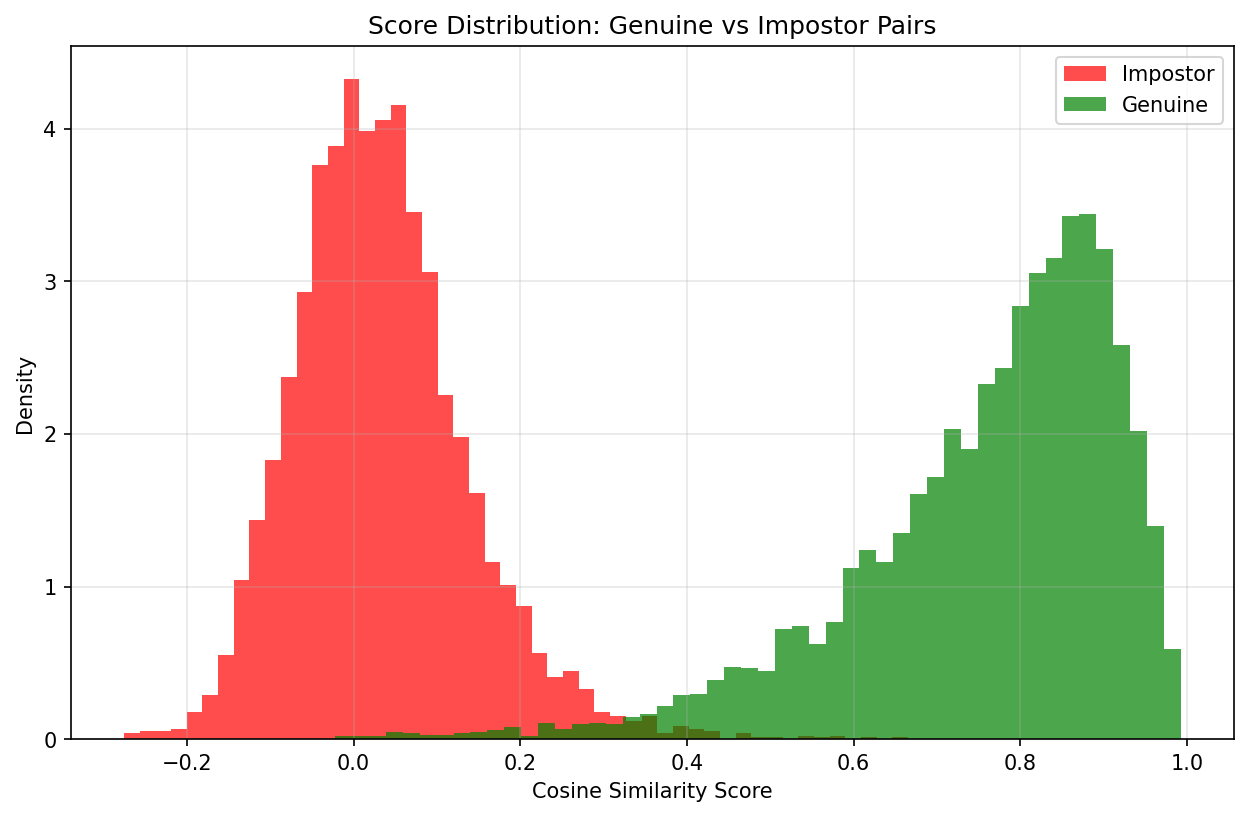
\includegraphics[width=\columnwidth]{score_dist_test.png}
\caption{Genuine (green) vs.\ impostor (red) cosine similarity score distributions on the test set. Clear separation enables reliable verification at a threshold of $\sim$0.30.}
\label{fig:scores}
\end{figure}

\begin{figure}[t]
\centering
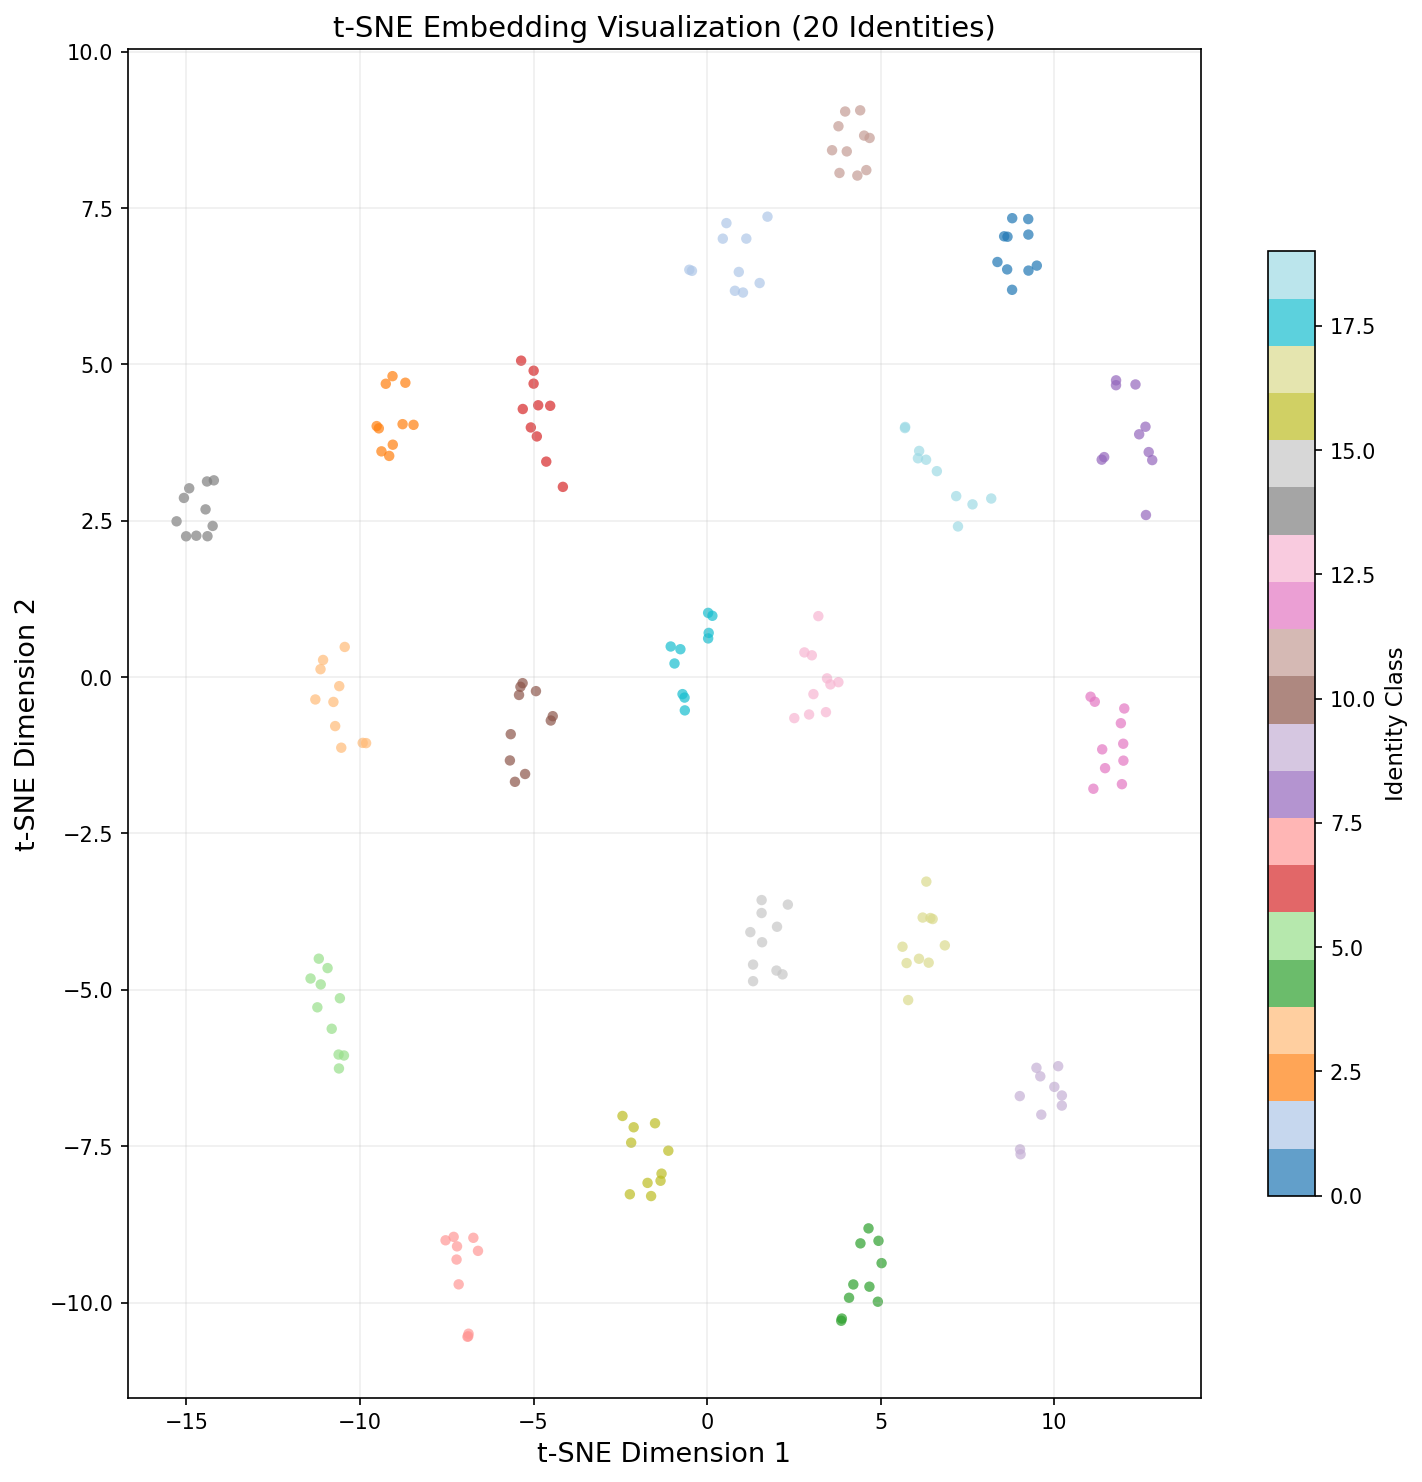
\includegraphics[width=\columnwidth]{tsne_embeddings.png}
\caption{t-SNE visualization of 256-D embeddings for 20 test identities. Tight, well-separated clusters confirm discriminative embedding learning.}
\label{fig:tsne}
\end{figure}

% ============================================================
\section{Baseline Implementation and Preliminary Results}

\subsection{Architecture}

Our model uses a two-stage architecture with approximately 12M parameters:

\begin{enumerate}
    \item \textbf{Backbone:} ResNet18~\cite{he2016deep} pretrained on ImageNet, with the final fully-connected layer replaced by an identity mapping, yielding 512-D feature vectors.
    \item \textbf{Projection Head:} A two-layer MLP ($512 \rightarrow 512 \rightarrow 256$) with batch normalization and ReLU, producing L2-normalized 256-D embeddings on the unit hypersphere.
\end{enumerate}

During training, an ArcFace~\cite{deng2019arcface} classification head computes $\text{logit}_j = s \cdot \cos(\theta_j + m \cdot \mathbb{1}[j = y])$ with scale $s = 30$ and angular margin $m = 0.3$. The ArcFace head is discarded at inference; only the embedder is used for verification via cosine similarity.

\subsection{Training}

The model is trained with AdamW (lr = $3 \times 10^{-4}$, weight decay = $10^{-3}$) and a cosine learning rate schedule for 50 epochs. Early stopping at epoch 42 selects the best checkpoint based on validation EER (1.13\% at epoch 32). Fig.~\ref{fig:training} shows the training convergence.

\begin{figure}[t]
\centering
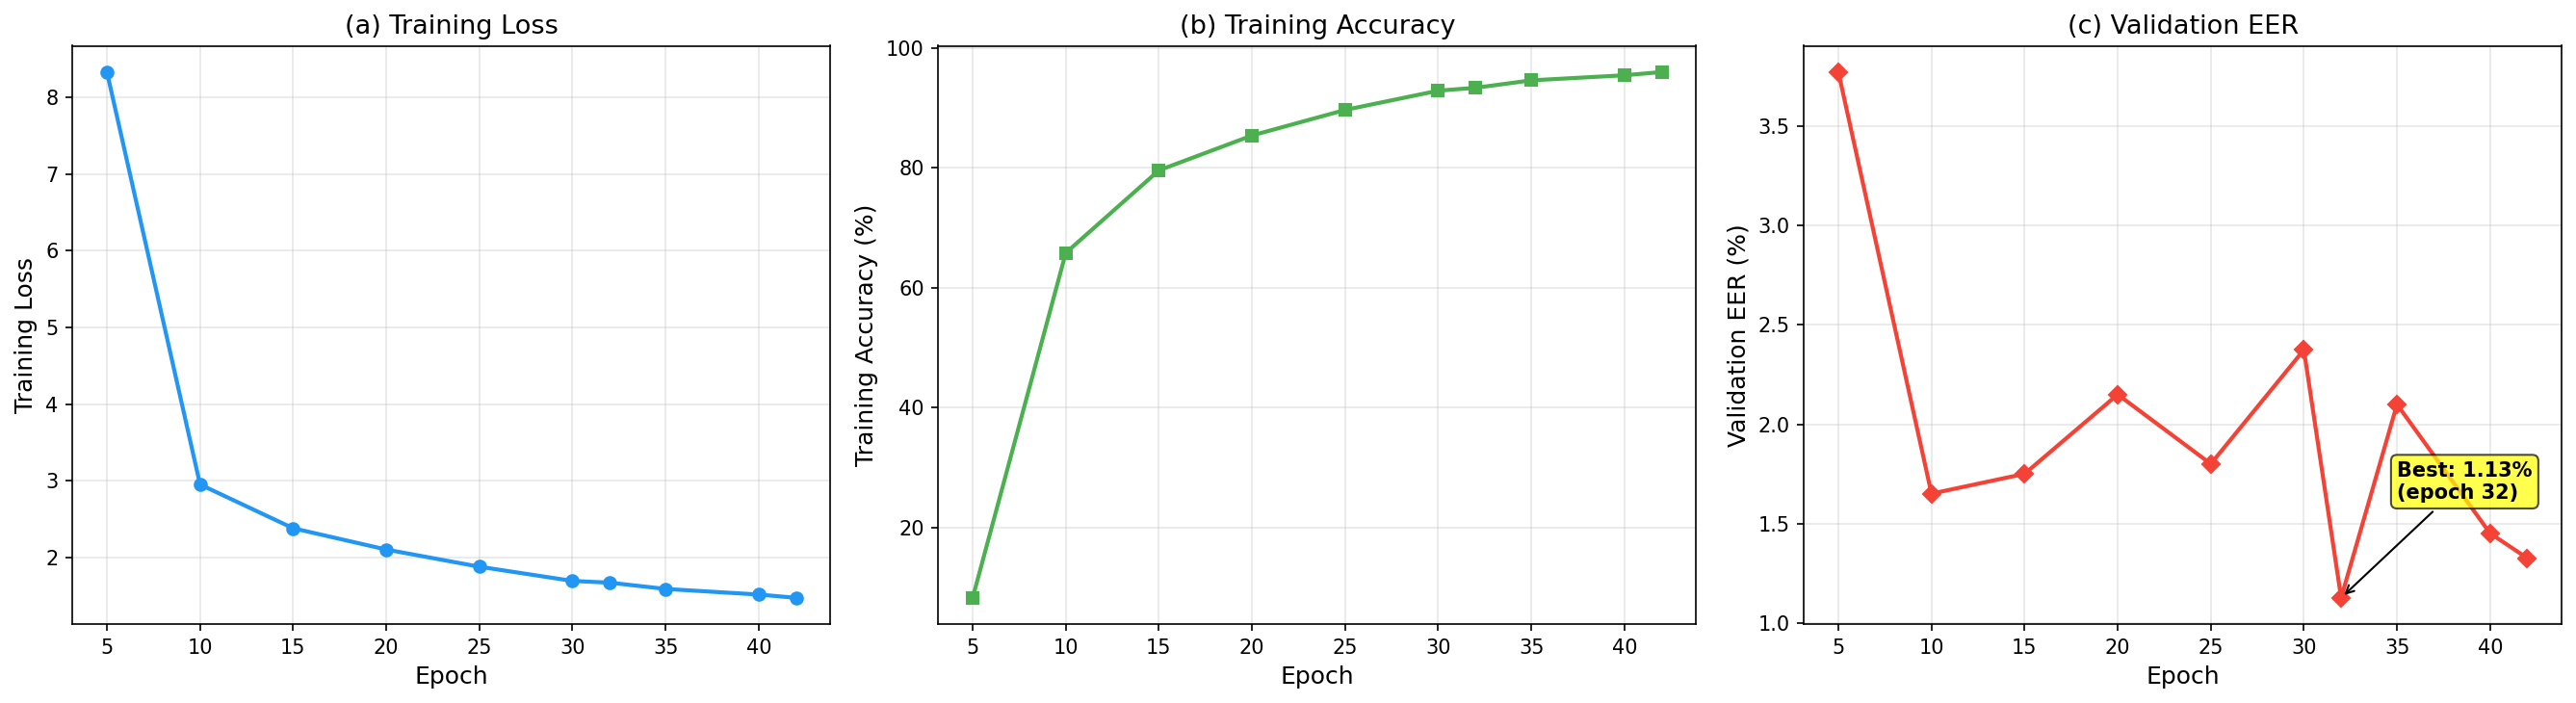
\includegraphics[width=\columnwidth]{training_curves.png}
\caption{Training convergence: (a) loss decreases from 8.3 to 1.5, (b) accuracy rises to 96\%, (c) validation EER reaches minimum 1.13\% at epoch 32.}
\label{fig:training}
\end{figure}

\subsection{Clean Test Performance}

Using the best checkpoint, we evaluate on the held-out test set (123 subjects, 246 classes, 2,460 images) with 5,000 genuine and 5,000 impostor pairs:

\begin{table}[h]
\centering
\caption{Verification metrics on clean test data.}
\label{tab:metrics}
\begin{tabular}{lc}
\toprule
\textbf{Metric} & \textbf{Value} \\
\midrule
EER                  & 1.67\% \\
FAR @ 1\% FRR        & 4.12\% \\
FAR @ 0.1\% FRR      & 48.88\% \\
Genuine mean sim.    & $0.759 \pm 0.160$ \\
Impostor mean sim.   & $0.033 \pm 0.105$ \\
\bottomrule
\end{tabular}
\end{table}

\subsection{Threshold and Error Analysis}

The EER operating point corresponds to a threshold of $\sim$0.30 on cosine similarity. The ROC curve (Fig.~\ref{fig:roc}) confirms strong discriminative performance with AUC exceeding 0.99. However, the high FAR @ 0.1\% FRR (48.88\%) reveals that genuine and impostor distributions have overlapping tails---at very strict operating points, the system cannot reliably separate all pairs. This tail overlap likely stems from limited intra-class variability in the training data ($\sim$10 images per class).

\begin{figure}[t]
\centering
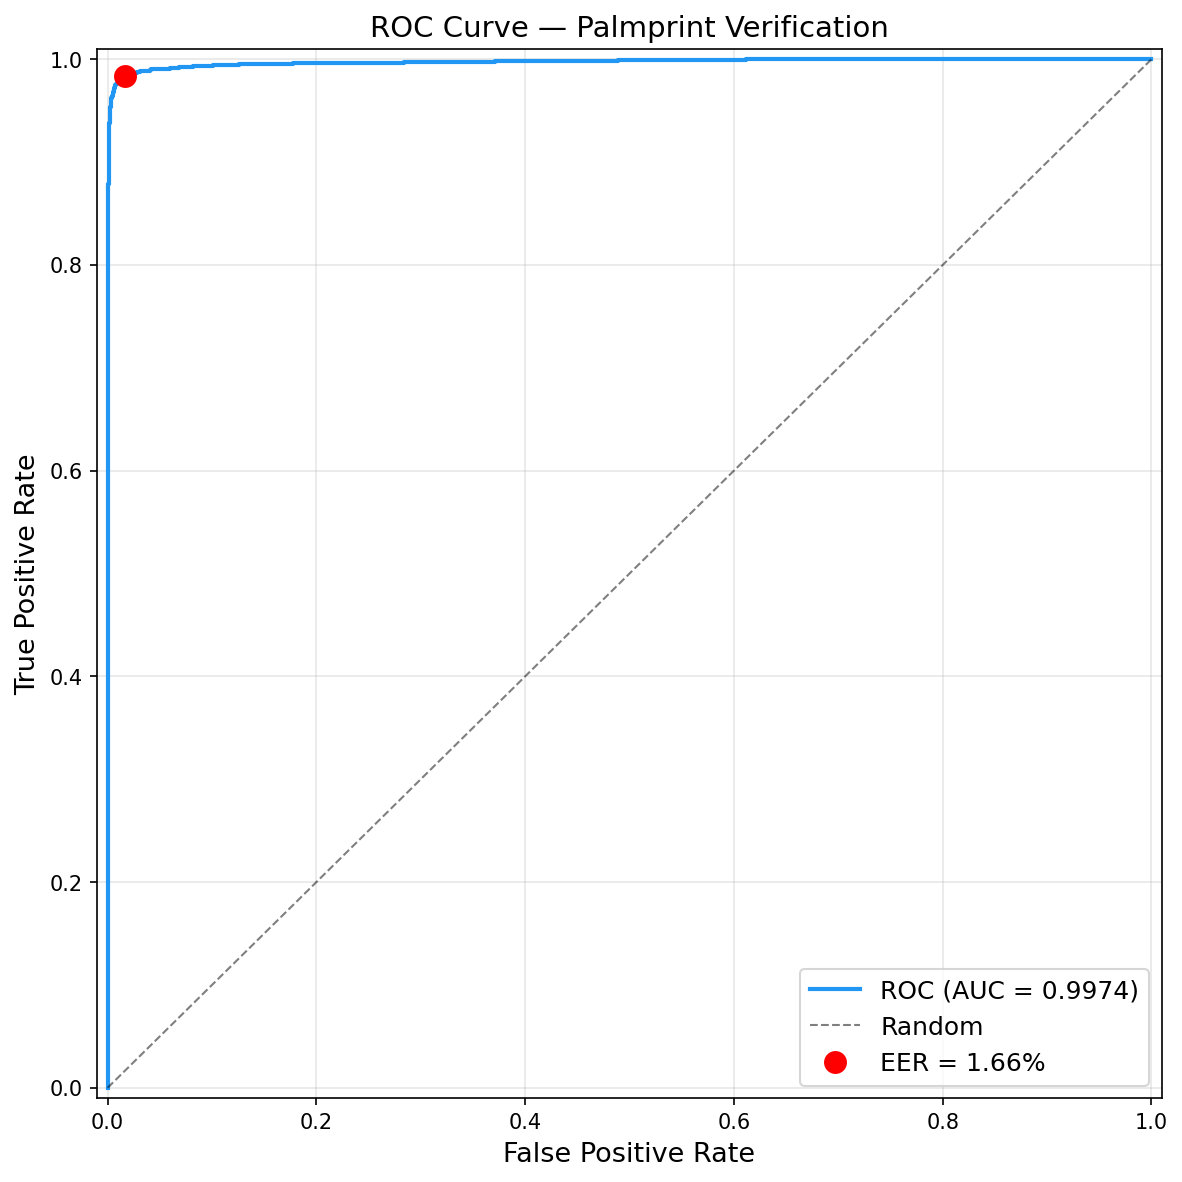
\includegraphics[width=\columnwidth]{roc_curve.png}
\caption{ROC curve with EER operating point (red dot). AUC $>$ 0.99 confirms strong baseline verification performance.}
\label{fig:roc}
\end{figure}

\subsection{Robustness Summary}

Our robustness benchmark evaluates the model under 9 corruption types at 5 severity levels (45 conditions). Table~\ref{tab:robustness} summarizes the results, ranked by worst-case degradation:

\begin{table}[h]
\centering
\caption{Robustness benchmark: EER degradation by corruption type.}
\label{tab:robustness}
\begin{tabular}{lccc}
\toprule
\textbf{Corruption} & \textbf{Mean EER} & \textbf{Worst EER} & \textbf{Degrad.} \\
\midrule
Noise        & 10.02\% & 21.90\% & +1,170\% \\
Motion Blur  & 8.46\%  & 19.67\% & +1,041\% \\
Brightness   & 6.85\%  & 15.45\% & +796\%   \\
JPEG         & 5.12\%  & 11.12\% & +545\%   \\
Rotation     & 5.01\%  & 9.15\%  & +430\%   \\
Occlusion    & 4.52\%  & 7.80\%  & +352\%   \\
Gauss.\ Blur & 2.85\%  & 4.45\%  & +158\%   \\
Scale        & 2.41\%  & 3.05\%  & +77\%    \\
Contrast     & 1.98\%  & 2.28\%  & +32\%    \\
\bottomrule
\end{tabular}
\end{table}

The three most damaging factors---noise, motion blur, and brightness---each cause $>$5$\times$ EER increase at maximum severity, presenting clear targets for mitigation in the final project phase.

% ============================================================
\section{Code Repository}

The complete source code is available at: \texttt{[GitHub link -- to be added]}.

\medskip
\noindent\textbf{Repository structure:}
\begin{itemize}
    \item \texttt{src/} -- Training, evaluation, and corruption scripts
    \item \texttt{splits/} -- Subject-disjoint split definitions (JSON)
    \item \texttt{figures/} -- Generated plots and visualizations
    \item \texttt{checkpoints/} -- Model weights and evaluation results
    \item \texttt{docs/} -- Proposal and report documents
    \item \texttt{requirements.txt} -- Python dependencies
    \item \texttt{README.md} -- Setup and usage instructions
\end{itemize}

% ============================================================
\bibliographystyle{IEEEtran}
\begin{thebibliography}{6}

\bibitem{polyu}
PolyU--IITD Contactless Palmprint Database v3.0, The Hong Kong Polytechnic University.

\bibitem{deng2019arcface}
J.~Deng, J.~Guo, N.~Xue, and S.~Zafeiriou, ``ArcFace: Additive angular margin loss for deep face recognition,'' in \textit{Proc. IEEE/CVF CVPR}, 2019, pp.~4690--4699.

\bibitem{he2016deep}
K.~He, X.~Zhang, S.~Ren, and J.~Sun, ``Deep residual learning for image recognition,'' in \textit{Proc. IEEE CVPR}, 2016, pp.~770--778.

\bibitem{hendrycks2019benchmarking}
D.~Hendrycks and T.~Dietterich, ``Benchmarking neural network robustness to common corruptions and perturbations,'' in \textit{Proc. ICLR}, 2019.

\bibitem{zhong2019palmprint}
D.~Zhong, X.~Du, and K.~Zhong, ``Decade progress of palmprint recognition: A brief survey,'' \textit{Neurocomputing}, vol.~328, pp.~16--28, 2019.

\bibitem{zhang2003palmcode}
D.~Zhang, W.-K.~Kong, J.~You, and M.~Wong, ``Online palmprint identification,'' \textit{IEEE Trans. Pattern Anal. Mach. Intell.}, vol.~25, no.~9, pp.~1041--1050, 2003.

\end{thebibliography}

\end{document}
